\documentclass{beamer}
\usepackage{tikz}
\usepackage{verbatim}
\usetheme{Warsaw}
\title{Intersection Management with Constraint-Based Reservation
System}
\author{Tsz-Chiu Au, Shun Zhang, Peter Stone\\ Department of Computer
Science\\ The University of Texas at Austin}

\defbeamertemplate*{footline}{shadow theme}
{%
  \leavevmode%
  \hbox{\begin{beamercolorbox}[wd=.5\paperwidth,ht=2.5ex,dp=1.125ex,leftskip=.3cm plus1fil,rightskip=.3cm]{author in head/foot}%
    \usebeamerfont{author in head/foot}\insertframenumber\,/\,\inserttotalframenumber\hfill\insertshortauthor
  \end{beamercolorbox}%
  \begin{beamercolorbox}[wd=.5\paperwidth,ht=2.5ex,dp=1.125ex,leftskip=.3cm,rightskip=.3cm plus1fil]{title in head/foot}%
    \usebeamerfont{title in head/foot}\insertshorttitle%
  \end{beamercolorbox}}%
}

\begin{document}

\begin{frame}
\titlepage
\end{frame}

\section{Introduction}

\subsection{Autonomous Intersection Management}

\begin{frame}{Transportation Infrastructure: Present and Future}
\begin{columns}[c]
	\column{.6\textwidth}
		\begin{itemize}
		\item Today’s transportation infrastructure is designed for
		human drivers.
		\item In the future: Autonomous Traffic Management\\
		Utilize the capacity of autonomous vehicles to improve traffic
		in transportation systems.
		\end{itemize}
		
	\column{.4\textwidth}
		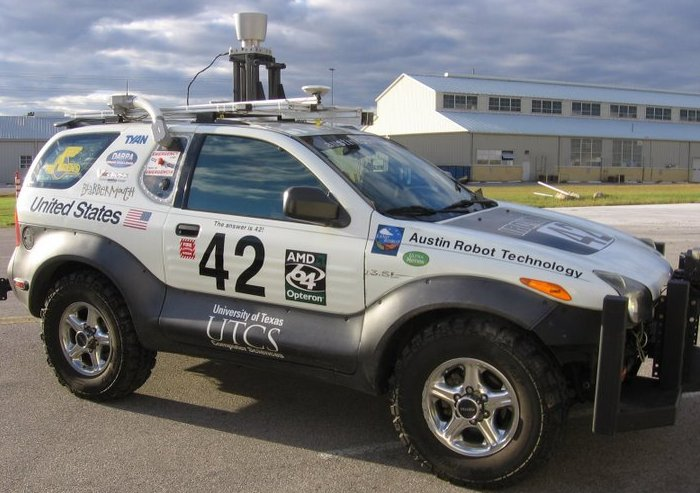
\includegraphics[width=0.8\textwidth]{42.png}
		\hfill
		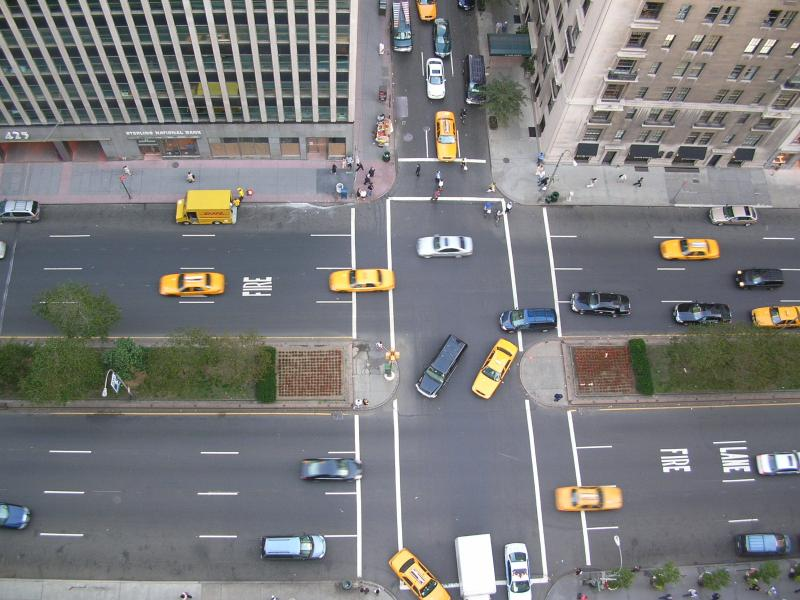
\includegraphics[width=0.8\textwidth]{intersection.jpg}
\end{columns}
\end{frame}

\begin{frame}{Autonomous Intersection Management}
\begin{columns}[c]
	\column{.4\textwidth}
		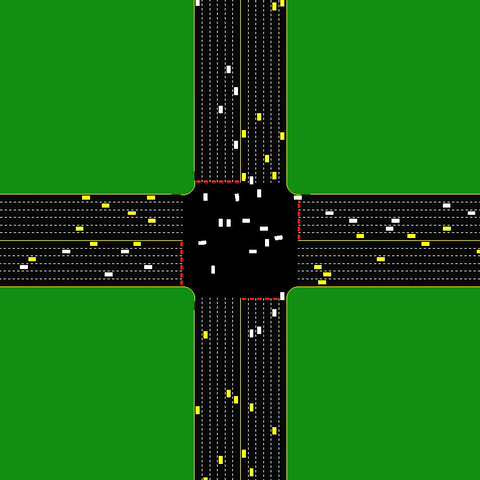
\includegraphics[width=\textwidth]{aim.png}
				
	\column{.6\textwidth}
		\begin{itemize}
		\item Dramatically reduce the traffic delay.
		\item Reduce the overhead of fuel consumption by approximately
		two thirds.\\
		Kurt Dresner and Peter Stone. A Multiagent Approach to
		Autonomous Intersection Management. JAIR 2008.
		\end{itemize}
\end{columns}
\end{frame}

\begin{frame}{Grid-Based Collision Detection}
	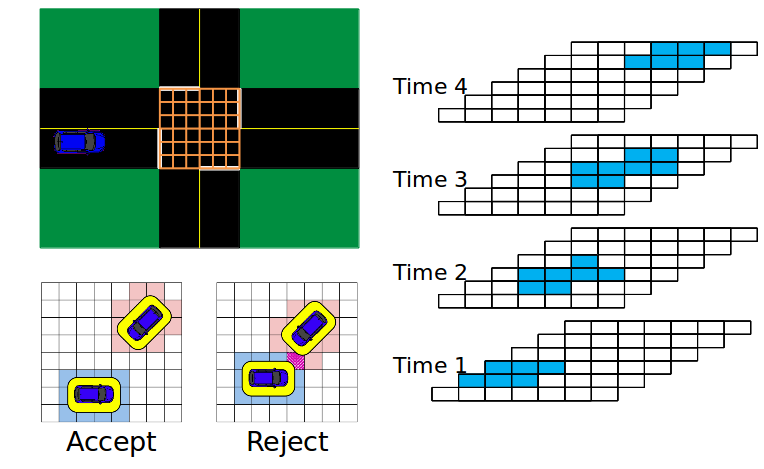
\includegraphics[width=\textwidth]{grids.png}
\end{frame}

\begin{frame}{Evaluation}
%	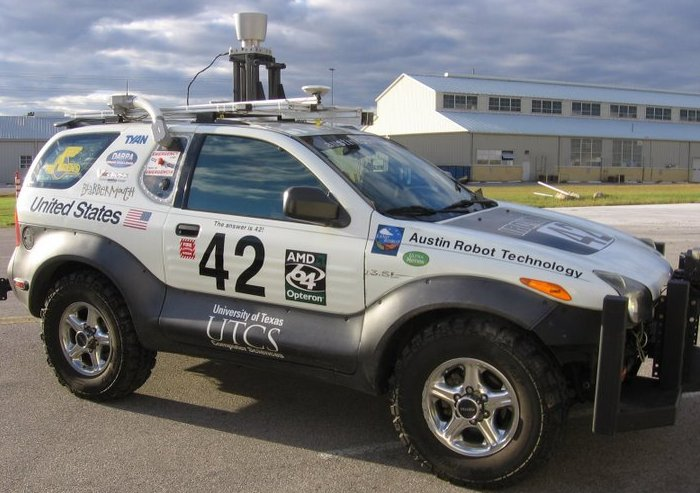
\includegraphics[width=0.8\textwidth]{42.png}
\end{frame}

\section{Semi-Autonomous Intersection Manangement}

\subsection{Motivation}

\begin{frame}{Sharing the Road with Human Drivers}
\begin{columns}[c]
\column{.6\textwidth}
\begin{itemize}
\item AIM is designed for the time when vehicles are autonomous.
\item Autonomous vehicles won’t displace manual-controlled vehicles in one
day. Some people enjoy driving.
\item One solution: FCFS-light = First-Come First-Served Policy + Traffic Signals
\end{itemize}
\column{.4\textwidth}
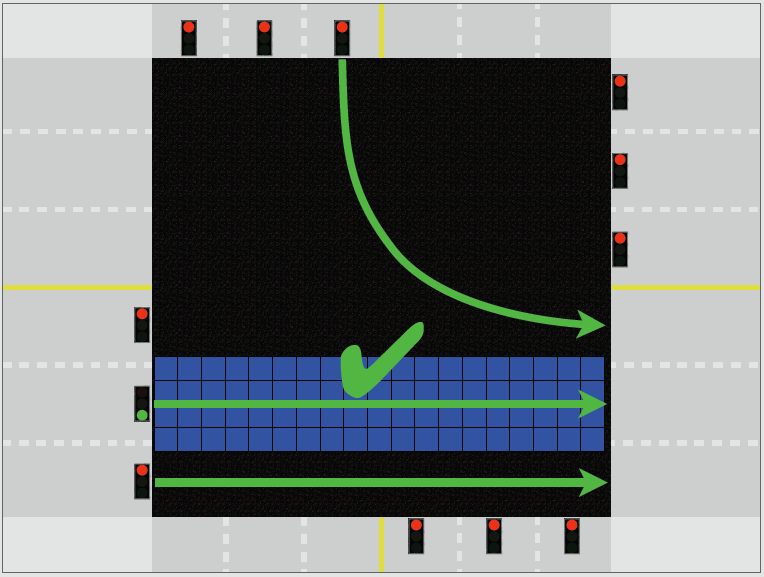
\includegraphics[width=\textwidth]{fcfs-light-1.png}
\hfill
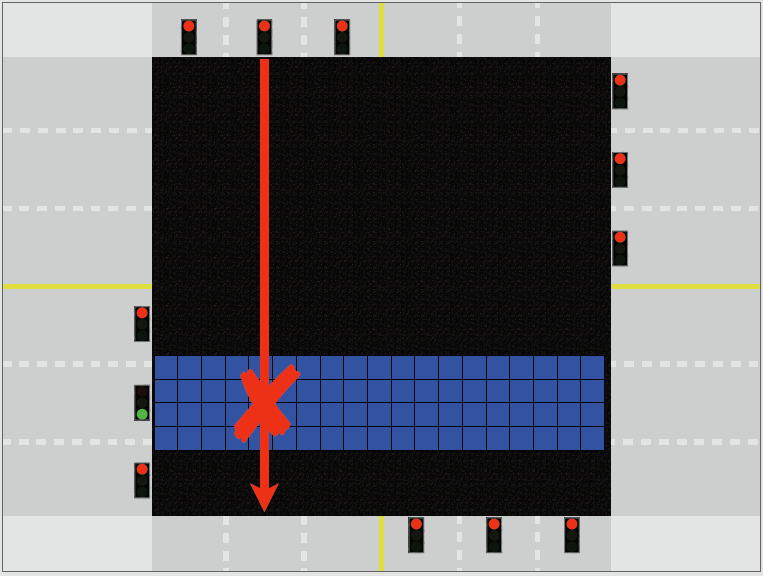
\includegraphics[width=\textwidth]{fcfs-light-2.png}
\end{columns}
\end{frame}

\subsection{Semi-Autonomous Vechiles}

\begin{frame}{Definition}
\textit{semi-autonomous vehicles}: vehicles with limited autonomous
driving and wireless communication capabilities.

\hfill

They are able to follow a limited number of predictable trajectories
at intersections more precisely than human drivers.
\end{frame}

\begin{frame}{Type of Semi-Autonomous Vehicles}
\begin{tabular}{|c|c|c|c|}
  \hline
  Vehicle Type & Communication & Cruise & Adaptive \\
               & Device & Control & Cruise Control \\
  \hline
  SA-ACC & X & X & X  \\
  \hline
  SA-CC & X & X &  \\
  \hline
  SA-Com & X & &  \\
  \hline
\end{tabular}
\end{frame}

\begin{frame}{Evaluations}
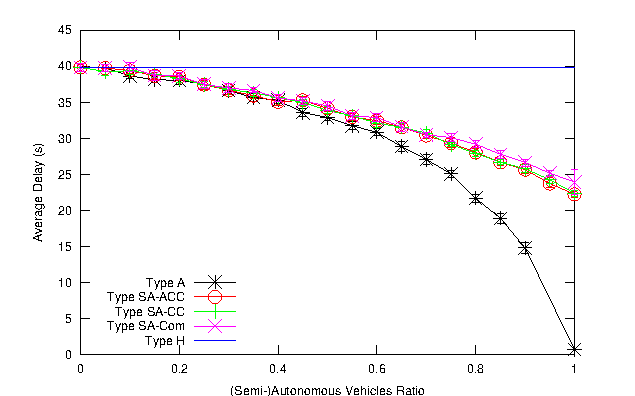
\includegraphics[width=0.9\textwidth]{figures/figure_1.pdf}

(Semi-)Autonomous vehicles vs. Human-Driven vehicles. Traffic
level = 360 vehicles/lane/hour.
\end{frame}

\subsection{Interaction Model}

\begin{frame}{Interaction Model}
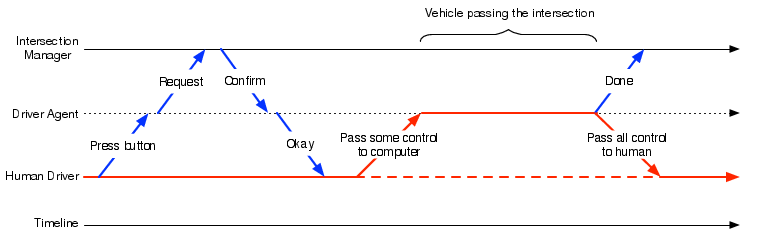
\includegraphics[width=\textwidth]{figures/interaction}
\end{frame}

\subsection{Constraint-based Reservation Systems}

\section{Conclusion}

\begin{frame}
\large{Thank you!}

\hfill
\hfill
\hfill

\tiny{Sources:

http://www.cs.utexas.edu/~pstone/Courses/394Rspring13/resources/index.html

http://www.cs.utexas.edu/~pstone/Courses/343spring12/resources/index.html}
\end{frame}

\end{document}
